
%(BEGIN_QUESTION)
% Copyright 2011, Tony R. Kuphaldt, released under the Creative Commons Attribution License (v 1.0)
% This means you may do almost anything with this work of mine, so long as you give me proper credit

A level control system uses a variable-frequency motor drive (VFD) to control the speed of a pump drawing liquid out of the vessel.  The greater the liquid level, the faster the pump spins, drawing liquid out at a faster rate.  A low-level cutoff switch is also part of this control system, forcing the pump to a full stop to protect it from running dry if ever a low-level condition is sensed by the switch:

$$\includegraphics[width=15.5cm]{i03235x01.eps}$$

Unfortunately, this system seems to have a problem.  The pump refuses to start even though the liquid level is greater than the controller's setpoint (as indicated by both the controller and the sightglass).  It was running just fine yesterday, and no technician has touched any of the components since then.

\filbreak

A fellow instrument technician helping you troubleshoot this problem decides to perform a simple test: he uses his multimeter (configured to measure DC current) as a ``jumper'' wire to momentarily short together terminals 5 and 7 on terminal strip TB13.  Still, the motor remains off and does not start up as it should.

\vskip 10pt

Identify the likelihood of each specified fault for this control system.  Consider each fault one at a time (i.e. no coincidental faults), determining whether or not each fault could independently account for {\it all} measurements and symptoms in this system.

% No blank lines allowed between lines of an \halign structure!
% I use comments (%) instead, so that TeX doesn't choke.

$$\vbox{\offinterlineskip
\halign{\strut
\vrule \quad\hfil # \ \hfil & 
\vrule \quad\hfil # \ \hfil & 
\vrule \quad\hfil # \ \hfil \vrule \cr
\noalign{\hrule}
%
% First row
{\bf Fault} & {\bf Possible} & {\bf Impossible} \cr
%
\noalign{\hrule}
%
% Another row
No AC power to VFD &  &  \cr
%
\noalign{\hrule}
%
% Another row
Controller has dead 4-20 mA output &  &  \cr
%
\noalign{\hrule}
%
% Another row
Level transmitter out of calibration &  &  \cr
%
\noalign{\hrule}
%
% Another row
Level switch contacts failed shorted &  &  \cr
%
\noalign{\hrule}
%
% Another row
Level switch contacts failed open &  &  \cr
%
\noalign{\hrule}
%
% Another row
250 ohm resistor failed open &  &  \cr
%
\noalign{\hrule}
%
% Another row
Cable between TB12 and TB13 failed open &  &  \cr
%
\noalign{\hrule}
%
% Another row
Cable between TB13 and LSL failed open &  &  \cr
%
\noalign{\hrule}
} % End of \halign 
}$$ % End of \vbox

\vskip 10pt

Also, explain why the ``jumper test'' was a very good first step to take.

\vskip 20pt \vbox{\hrule \hbox{\strut \vrule{} {\bf Suggestions for Socratic discussion} \vrule} \hrule}

\begin{itemize}
\item{} Propose a ``next test'' to perform on this system to further isolate where the fault is located.
\item{} Is this an example of a {\it soft-constraint} override system or a {\it hard-constraint} override system?
\item{} Predict the effects resulting from various wiring faults in this system (e.g. {\it opens} or {\it shorts}).
\item{} What does the label {\it normally open} (NO) mean for a switch such as the one sensing liquid level here?
\item{} For those who have studied PID tuning, how should the level controller be tuned: mostly using proportional action, integral action, or derivative action to control the liquid level?
\end{itemize}

\underbar{file i03235}
%(END_QUESTION)





%(BEGIN_ANSWER)

% No blank lines allowed between lines of an \halign structure!
% I use comments (%) instead, so that TeX doesn't choke.

$$\vbox{\offinterlineskip
\halign{\strut
\vrule \quad\hfil # \ \hfil & 
\vrule \quad\hfil # \ \hfil & 
\vrule \quad\hfil # \ \hfil \vrule \cr
\noalign{\hrule}
%
% First row
{\bf Fault} & {\bf Possible} & {\bf Impossible} \cr
%
\noalign{\hrule}
%
% Another row
No AC power to VFD & $\surd$ &  \cr
%
\noalign{\hrule}
%
% Another row
Controller has dead 4-20 mA output & $\surd$ &  \cr
%
\noalign{\hrule}
%
% Another row
Level transmitter out of calibration &  & $\surd$ \cr
%
\noalign{\hrule}
%
% Another row
Level switch contacts failed shorted &  & $\surd$ \cr
%
\noalign{\hrule}
%
% Another row
Level switch contacts failed open &  & $\surd$ \cr
%
\noalign{\hrule}
%
% Another row
250 ohm resistor failed open &  & $\surd$ \cr
%
\noalign{\hrule}
%
% Another row
Cable between TB12 and TB13 failed open & $\surd$ &  \cr
%
\noalign{\hrule}
%
% Another row
Cable between TB13 and LSL failed open &  & $\surd$ \cr
%
\noalign{\hrule}
} % End of \halign 
}$$ % End of \vbox

%(END_ANSWER)





%(BEGIN_NOTES)

If the jumper test had indeed resulted in the motor starting up, it would have confirmed an open fault in either the level switch or in the cable connecting the switch to TB13.  It was a very easy test to perform, and did not even require a meter (any piece of wire would have done the trick just as well).  

Just because a test did not give dramatic results, does not mean it is not a good test!

\vfil \eject

\noindent
{\bf Summary Quiz:}

Identify the effect of a wire break at terminal 7 on TB-13:

$$\includegraphics[width=15.5cm]{i03235x01.eps}$$

\begin{itemize}
\item{} The pump may become damaged from running dry
\vskip 5pt 
\item{} The controller will indicate -25\% tank level 
\vskip 5pt 
\item{} The controller will indicate 0\% tank level
\vskip 5pt 
\item{} The motor will immediately go to full speed
\vskip 5pt 
\item{} The motor will immediately stop running
\vskip 5pt 
\item{} A fuse will blow on the 480 VAC lines
\end{itemize}


%INDEX% Basics, control loop troubleshooting: determining cause of control problem
%INDEX% Troubleshooting review: electric circuits

%(END_NOTES)


